\section{Афанасьев. Задание 3}

\textbf{Постановка задачи:}
Взять прямоугольный импульс, разложить его в ряд Фурье,
произвести изменения в спектре, выполнить обратное преобразование
Фурье, продемонстрировать результаты.
Произвести следующие изменения в спектре:

\begin{enumerate}
  \item Убрать гармонику с нулевой частотой (постоянную составляющую);
  \item Последовательно убирать гармоники с наименьшей частотой.
\end{enumerate}

\textbf{Решение:}
Для большей наглядности воспользуемся тригонометрической формой
преобразования Фурье и установим период сигнала $T=2 \pi$,
скважность равной двум, амплитуду равной единице
(см. формулу \ref{formula:AfanasyevNN.s(x)}).
   
\begin{equation}
\label{formula:AfanasyevNN.s(x)}
s(x)=
\begin{cases}
1, & 0 \leq x \leq \pi \\
0, & \pi < x \leq 2 \pi
\end{cases}
\end{equation}

Вычислим коэффициенты $a_0$, $a_n$ и $b_n$:
$$
a_0= \frac{1}{ \pi} \int_{- \pi}^{ \pi}{s(x) dx}=
\frac{1}{ \pi} \int_{0}^{ \pi}{1 dx}=
\frac{1}{ \pi} x= \bigg |_{0}^{ \pi}=1
$$

$$
a_n= \frac{1}{ \pi} \int_{- \pi}^{ \pi}{s(x) cos(n x) dx}=
\frac{1}{ \pi} \int_{0}^{ \pi}{cos(n x) dx}=
\begin{vmatrix}
t=n x \\
dt=t' dx=n dx \\
dx= \frac{dt}{n} \\
a=n \cdot 0=0 \\
b=n \cdot \pi=n \pi 
\end{vmatrix}=
$$
$$
= \frac{1}{n \pi} \int_{0}^{n \pi}{ cos(t) dt}=
\frac{1}{n \pi} sin(t) \bigg |_{0}^{n \pi}=
\frac{1}{n \pi} (sin(n \pi) - sin(0))=0
$$

$$
b_n= \frac{1}{ \pi} \int_{- \pi}^{ \pi}{s(x) sin(n x) dx}=
\frac{1}{ \pi} \int_{0}^{ \pi}{sin(n x) dx}=
\begin{vmatrix}
t=n x \\
dt=t' dx=n dx \\
dx= \frac{dt}{n} \\
a=n \cdot 0=0 \\
b=n \cdot \pi=n \pi 
\end{vmatrix}=
$$
$$
= \frac{1}{n \pi} \int_{0}^{n \pi}{ sin(t) dt}=
- \frac{1}{n \pi} cos(t) \bigg |_{0}^{n \pi}=
- \frac{1}{n \pi} (cos(n \pi) - cos(0))=
$$
$$
=
\begin{cases}
0, & n=2 k, k=(1,2,3, \cdots) \\
\frac{2}{n \pi}, & n=2 k + 1, k=(0,1,2,3, \cdots)
\end{cases}
$$

Таким образом прямоугольный импульс $s(x)$ раскладывается следующим образом:
$$
s(x) \sim \frac{a_0}{2} + \sum_{n=1}^{+ \infty}{a_n cos(n x) + b_n sin(n x)}=
\frac{1}{2} + \sum_{k=0}^{+ \infty}{ \frac{2 sin((2 k + 1) x)}{(2 k + 1) \pi}}
$$

Для построения графика спектра сигнала (см. рис. \ref{fig:AfanasyevMM.spectrum})
необходимо вычислить амплитуды каждой гармоники $A_0= \frac{a_0}{2},
A_n= \sqrt{a_n^2+b_n^2}, n=(1,2,3, \cdots)$.
На оси абсцисс нужно отложить $n=(0,1,2, \cdots)$, а на оси ординат значения $A_n$.


\begin{figure}[h]
	\centering
	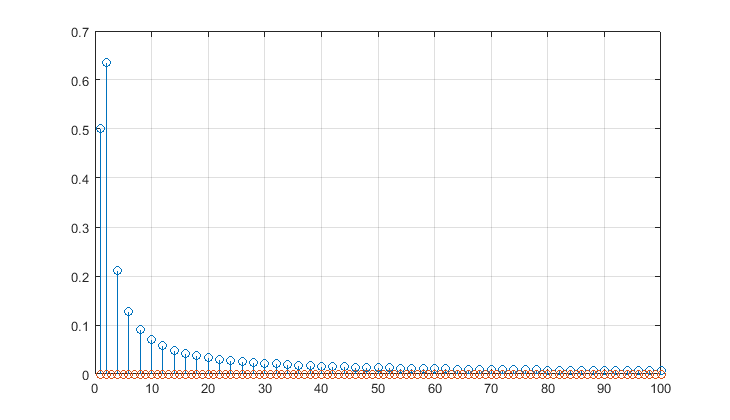
\includegraphics[width=0.9\linewidth]{AfanasyevMM/img/spectrum}
	\caption{Спектр сигнала $s(x)$}
	\label{fig:AfanasyevMM.spectrum}
\end{figure}


Обозначим через $f_i$ i-ую гармонику сигнала $s(x)$ и получим:
$$
s(x) \sim \sum_{i=0}^{+ \infty}{f_i}
$$
где $f_0= \frac{a_0}{2},
f_1= \frac{2 sin(x)}{ \pi},
f_2= 0,
f_3= \frac{2 sin(3 x)}{3 \pi},
f_4= 0,
f_5= \frac{2 sin(5 x)}{5 \pi},
\cdots$.

Обратное преобразование Фурье заключается в том, чтобы выполнить 
сложение $m$ гармоник, т.е. $s_{m}(x) \sim \sum_{i=0}^{m - 1}{f_i}, m > 0$.
Чем больше будет $m$, тем точнее будет воспроизведен прямоугольный
импульс $s(x)$.
На рисунках
\ref{fig:AfanasyevMM.s(x)_m1}, 
\ref{fig:AfanasyevMM.s(x)_m3},
\ref{fig:AfanasyevMM.s(x)_m5},
\ref{fig:AfanasyevMM.s(x)_m7},
\ref{fig:AfanasyevMM.s(x)_m21},
\ref{fig:AfanasyevMM.s(x)_m99}
продемонстрирован результат обратноого преобразование Фурье для разных
значений $m$.
На рисунках
\ref{fig:AfanasyevMM.s(x)_m100_d1}, 
\ref{fig:AfanasyevMM.s(x)_m100_d3},
\ref{fig:AfanasyevMM.s(x)_m100_d5},
\ref{fig:AfanasyevMM.s(x)_m100_d21},
\ref{fig:AfanasyevMM.s(x)_m100_d61}
продемонстрирован результат обратного преобразования Фурье для
$s_{m}(x) - s_{d}(x), d < m$. Код matlab, с помощью которого
были построены эти графики смотрите в листинге
\ref{code:AfanasyevMM.trigonometric_fourier}.

Таким образом видно, что $f_0$ задает постоянный уровень относительно
которого коллеблются остальные гармоники $f_i$, а сами $f_i$ уже формируют
форму сигнала.

\begin{figure}[H]
	\centering
	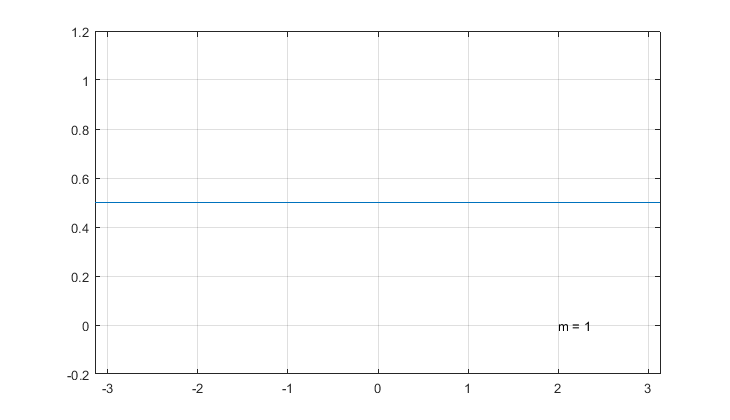
\includegraphics[width=0.5\linewidth]{AfanasyevMM/img/s(x)_m1}
	\caption{$s_{1}(x)$}
	\label{fig:AfanasyevMM.s(x)_m1}
\end{figure}
\begin{figure}[H]
	\centering
	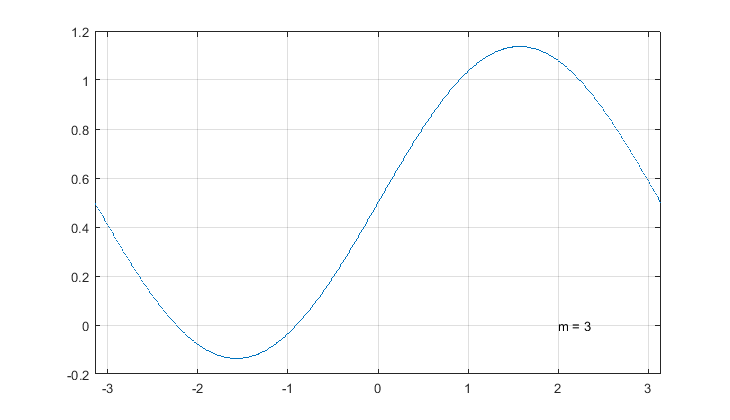
\includegraphics[width=0.5\linewidth]{AfanasyevMM/img/s(x)_m3}
	\caption{$s_{3}(x)$}
	\label{fig:AfanasyevMM.s(x)_m3}
\end{figure}
\begin{figure}[H]
	\centering
	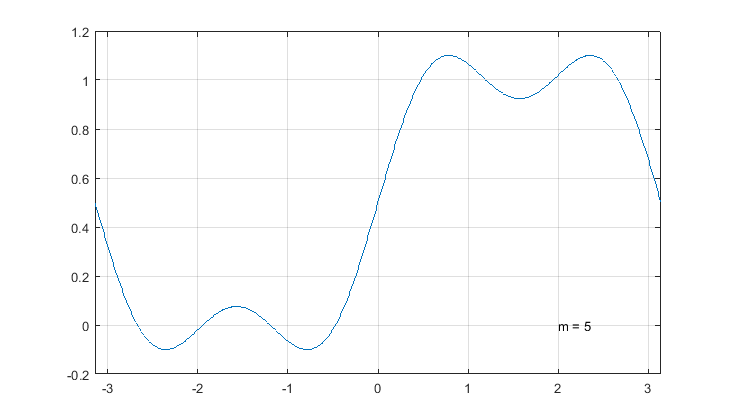
\includegraphics[width=0.5\linewidth]{AfanasyevMM/img/s(x)_m5}
	\caption{$s_{5}(x)$}
	\label{fig:AfanasyevMM.s(x)_m5}
\end{figure}
\begin{figure}[H]
	\centering
	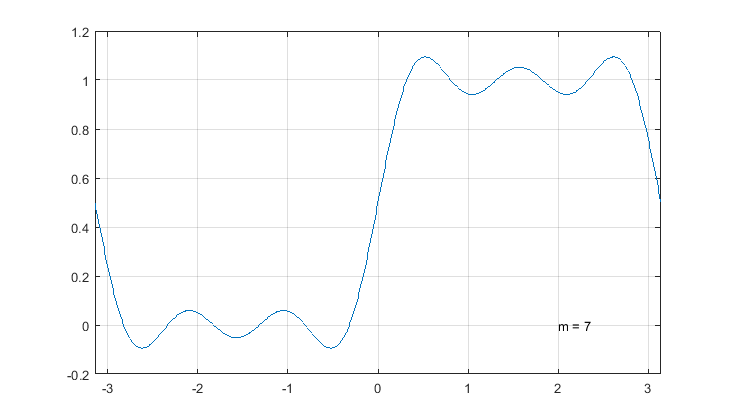
\includegraphics[width=0.5\linewidth]{AfanasyevMM/img/s(x)_m7}
	\caption{$s_{7}(x)$}
	\label{fig:AfanasyevMM.s(x)_m7}
\end{figure}
\begin{figure}[H]
	\centering
	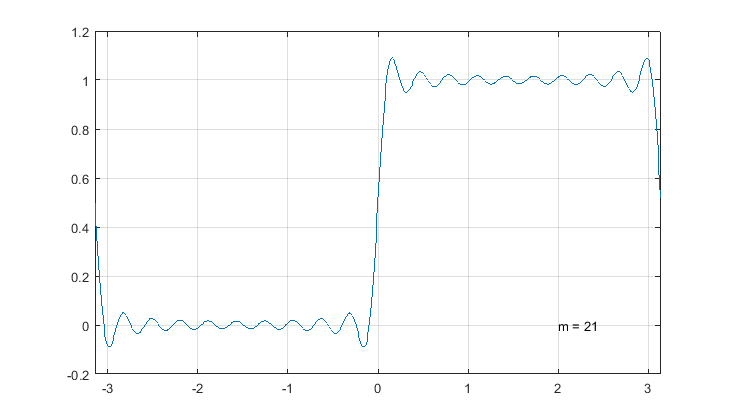
\includegraphics[width=0.5\linewidth]{AfanasyevMM/img/s(x)_m21}
	\caption{$s_{21}(x)$}
	\label{fig:AfanasyevMM.s(x)_m21}
\end{figure}
\begin{figure}[H]
	\centering
	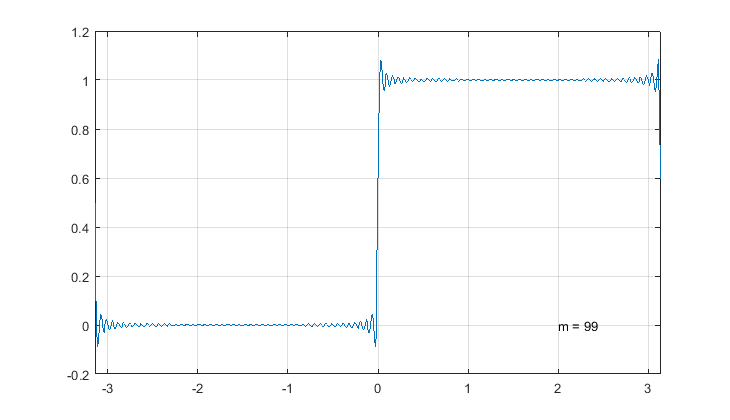
\includegraphics[width=0.5\linewidth]{AfanasyevMM/img/s(x)_m99}
	\caption{$s_{99}(x)$}
	\label{fig:AfanasyevMM.s(x)_m99}
\end{figure}
\begin{figure}[H]
	\centering
	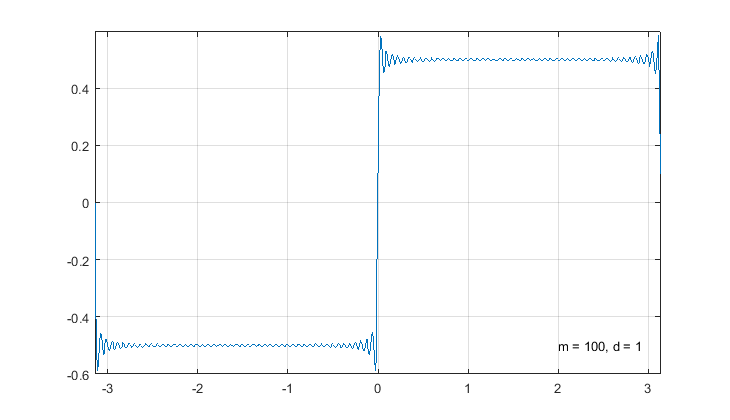
\includegraphics[width=0.5\linewidth]{AfanasyevMM/img/s(x)_m100_d1}
	\caption{$s_{100}(x) - s_{1}(x)$}
	\label{fig:AfanasyevMM.s(x)_m100_d1}
\end{figure}
\begin{figure}[H]
	\centering
	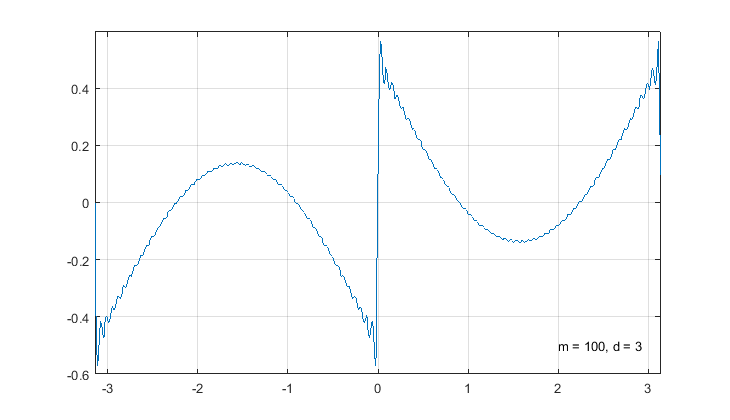
\includegraphics[width=0.5\linewidth]{AfanasyevMM/img/s(x)_m100_d3}
	\caption{$s_{100}(x) - s_{3}(x)$}
	\label{fig:AfanasyevMM.s(x)_m100_d3}
\end{figure}
\begin{figure}[H]
	\centering
	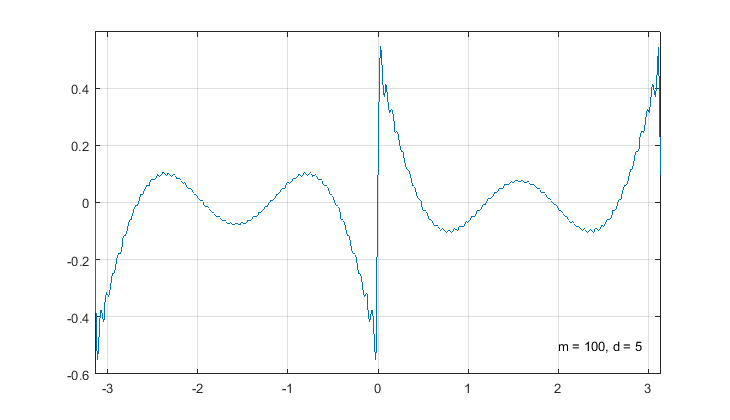
\includegraphics[width=0.5\linewidth]{AfanasyevMM/img/s(x)_m100_d5}
	\caption{$s_{100}(x) - s_{5}(x)$}
	\label{fig:AfanasyevMM.s(x)_m100_d5}
\end{figure}
\begin{figure}[H]
	\centering
	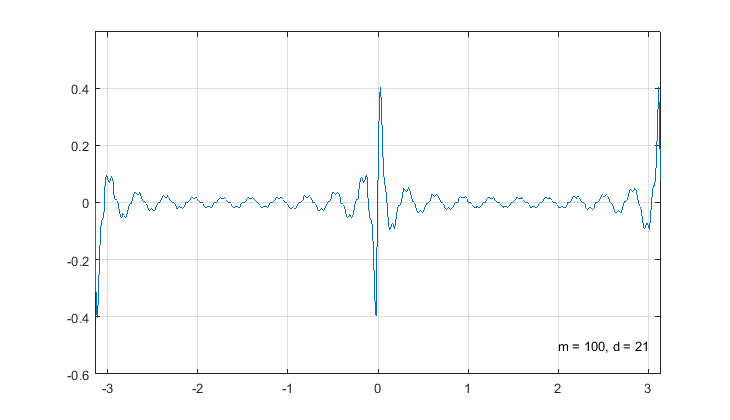
\includegraphics[width=0.5\linewidth]{AfanasyevMM/img/s(x)_m100_d21}
	\caption{$s_{100}(x) - s_{21}(x)$}
	\label{fig:AfanasyevMM.s(x)_m100_d21}
\end{figure}
\begin{figure}[H]
	\centering
	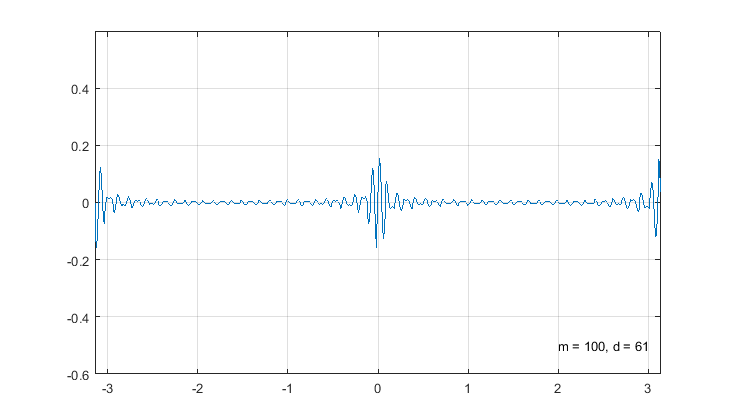
\includegraphics[width=0.5\linewidth]{AfanasyevMM/img/s(x)_m100_d61}
	\caption{$s_{100}(x) - s_{61}(x)$}
	\label{fig:AfanasyevMM.s(x)_m100_d61}
\end{figure}
\lstset{language=Matlab,
        basicstyle=\small}
%\label{code:AfanasyevMM.trigonometric_fourier}
\lstinputlisting[language=Matlab, frame=single,
label=code:AfanasyevMM.trigonometric_fourier, caption=Листинг программы]
{AfanasyevMM/src/trigonometric_fourier.m}
\newpage